\sectionframe{What is Period-adding?}
\section{Period-adding?}

\begin{frame}{Period-adding}
	\vspace{-1em}
	\begin{columns}
		\begin{column}{.5 \textwidth}
			\begin{figure}
				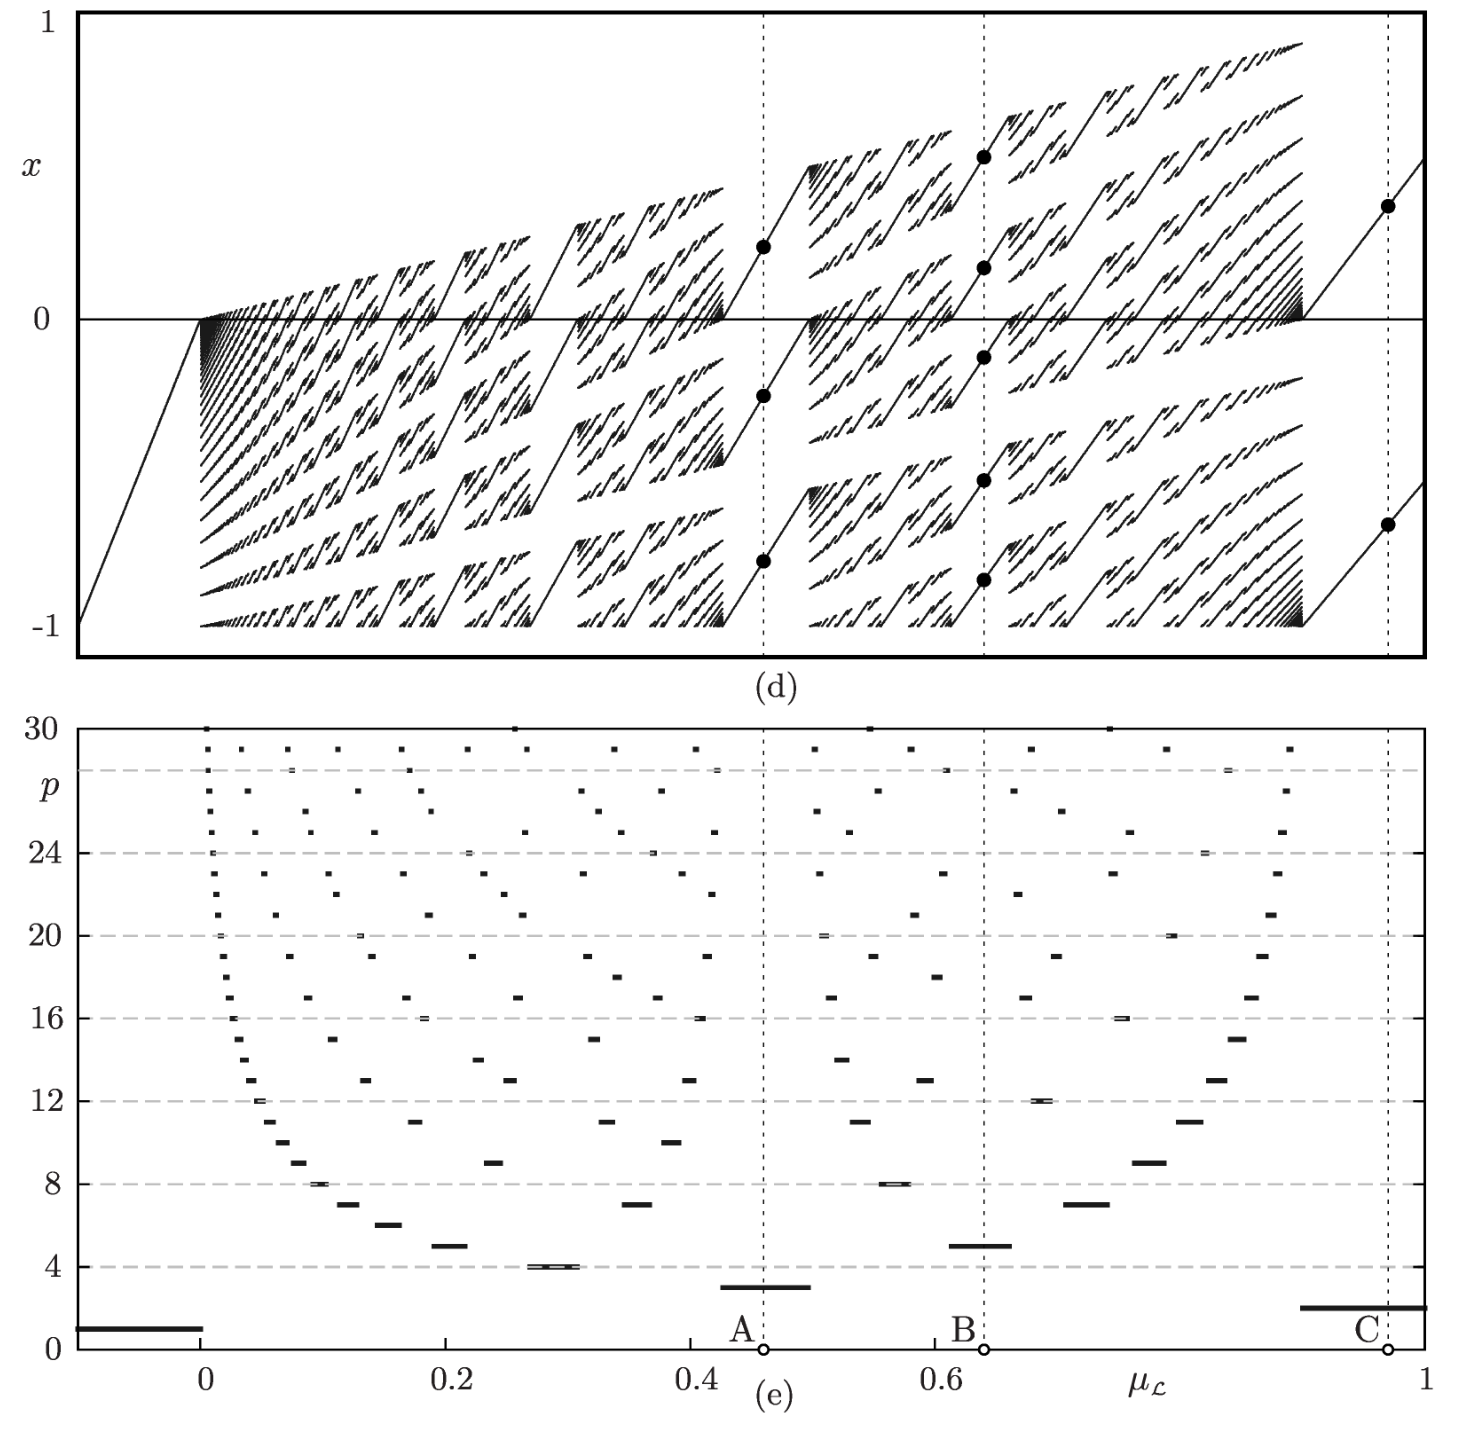
\includegraphics[width=.8 \textwidth]{Figs/PeriodAddingDiagrams_Slides.png}
			\end{figure}
		\end{column}
		\begin{column}{.5 \textwidth}
			\only<2->{
				\begin{figure}
					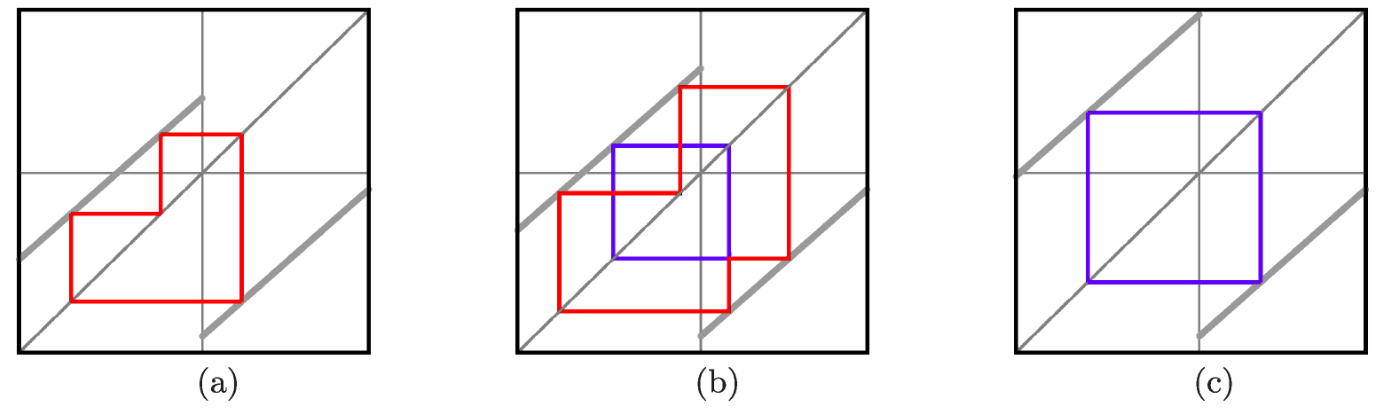
\includegraphics[width=\textwidth]{Figs/PeriodAddingCobwebs_Slides.png}
				\end{figure}
				\begin{itemize}
					\item Between two cycles with periods $a$ and $b$ there is a cycle with period $a + b$
					      \pause
					\item How are these cycles organized?
				\end{itemize}
			}
		\end{column}
	\end{columns}
\end{frame}

\begin{frame}{A Seemingly Unrelated Concept}
	Farey-sequences
	\begin{itemize}
		\item First discovered by Charles Haros in 1802
		\item Rediscovered by and named after John Farey in 1816
		      \pause
		\item Also used by Louis-Achille Brocot, a french clock-maker
		\item Dealing with gear ratios
		      \pause
		\item Possible connection: Gears have a discrete number of teeth \\
		      and cycles have a discrete number of points
	\end{itemize}
\end{frame}

\begin{frame}{Farey-sequences}
	\vspace{-1em}
	\begin{definition}[Farey-sequences]
		The Farey-sequence $\F^m$ of order $m$ is defined as the set of irreducible fractions in the closed interval $[0, 1]$
		with denominators not larger than $m$, listed in increasing order.
	\end{definition}
	\pause
	\begin{itemize}
		\item $\F^1 = \left\{ \frac{0}{1}, \frac{1}{1} \right\}$ \vspace{.1em}
		\item $\F^2 = \left\{ \frac{0}{1}, \frac{1}{2}, \frac{1}{1} \right\}$ \vspace{.1em}
		\item $\F^3 = \left\{ \frac{0}{1}, \frac{1}{3}, \frac{1}{2}, \frac{2}{3}, \frac{1}{1} \right\}$
	\end{itemize}
	\pause
	\begin{theorem}[Farey-addition]
		Let $\frac{a_1}{b_1}, \frac{a_2}{b_2},$ and $\frac{a_3}{b_3}$ be 3 consecutive terms of $\F^m$. Then
		\begin{align*}
			\frac{a_2}{b_2} = \frac{a_1}{b_1} \oplus \frac{a_3}{b_3} = \frac{a_1 + a_3}{b_1 + b_3}
		\end{align*}
	\end{theorem}
\end{frame}

\begin{frame}{Farey-trees}
	\begin{columns}
		\begin{column}{.5 \textwidth}
			\vspace{-2em}
			\begin{itemize}
				\item Tool to visualize and construct Farey-sequences
				\item Child node holds mediant (Farey-sum) of values in parent nodes
				      \pause
				      \vspace{1em}
				\item Contains all rational numbers in $[0, 1]$
				\item Numbers monotonously increasing
			\end{itemize}
			\vspace{-.7em}
			\only<3>{
				\begin{figure}
					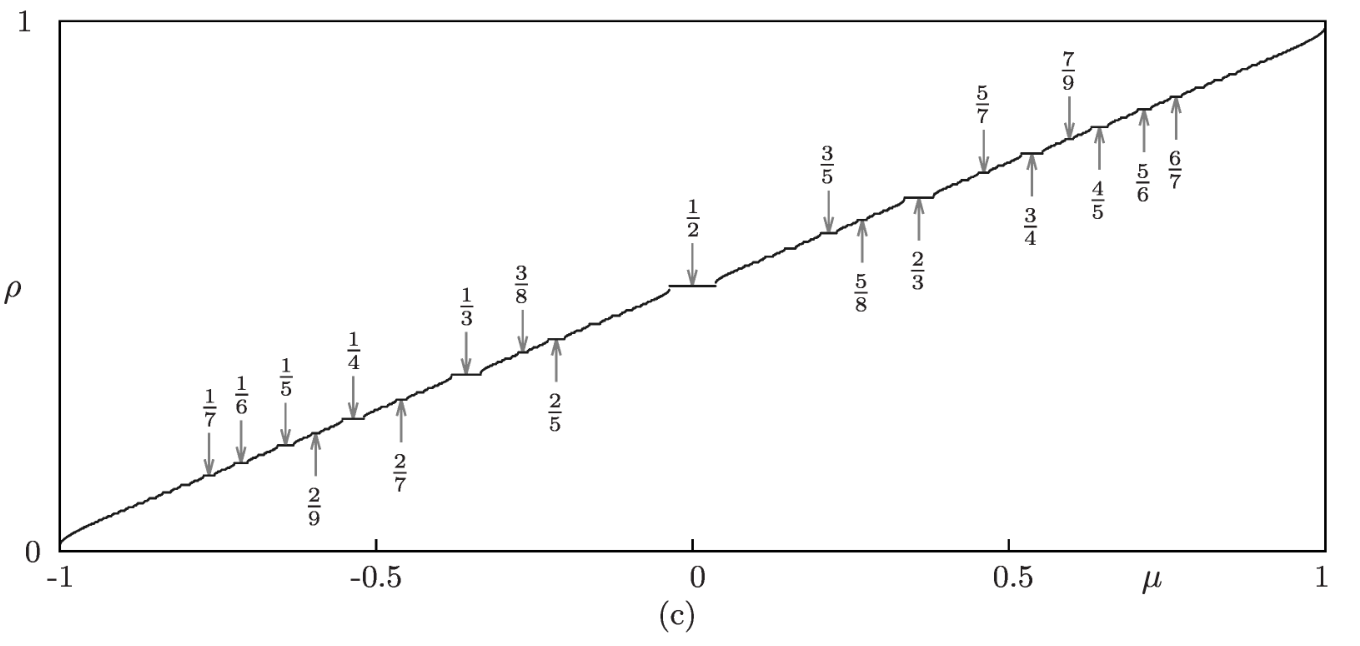
\includegraphics[width=\textwidth]{Figs/devils_staircase.png}
				\end{figure}
			}
		\end{column}
		\begin{column}{.5 \textwidth}
			\vspace{-5em}
			\begin{figure}
				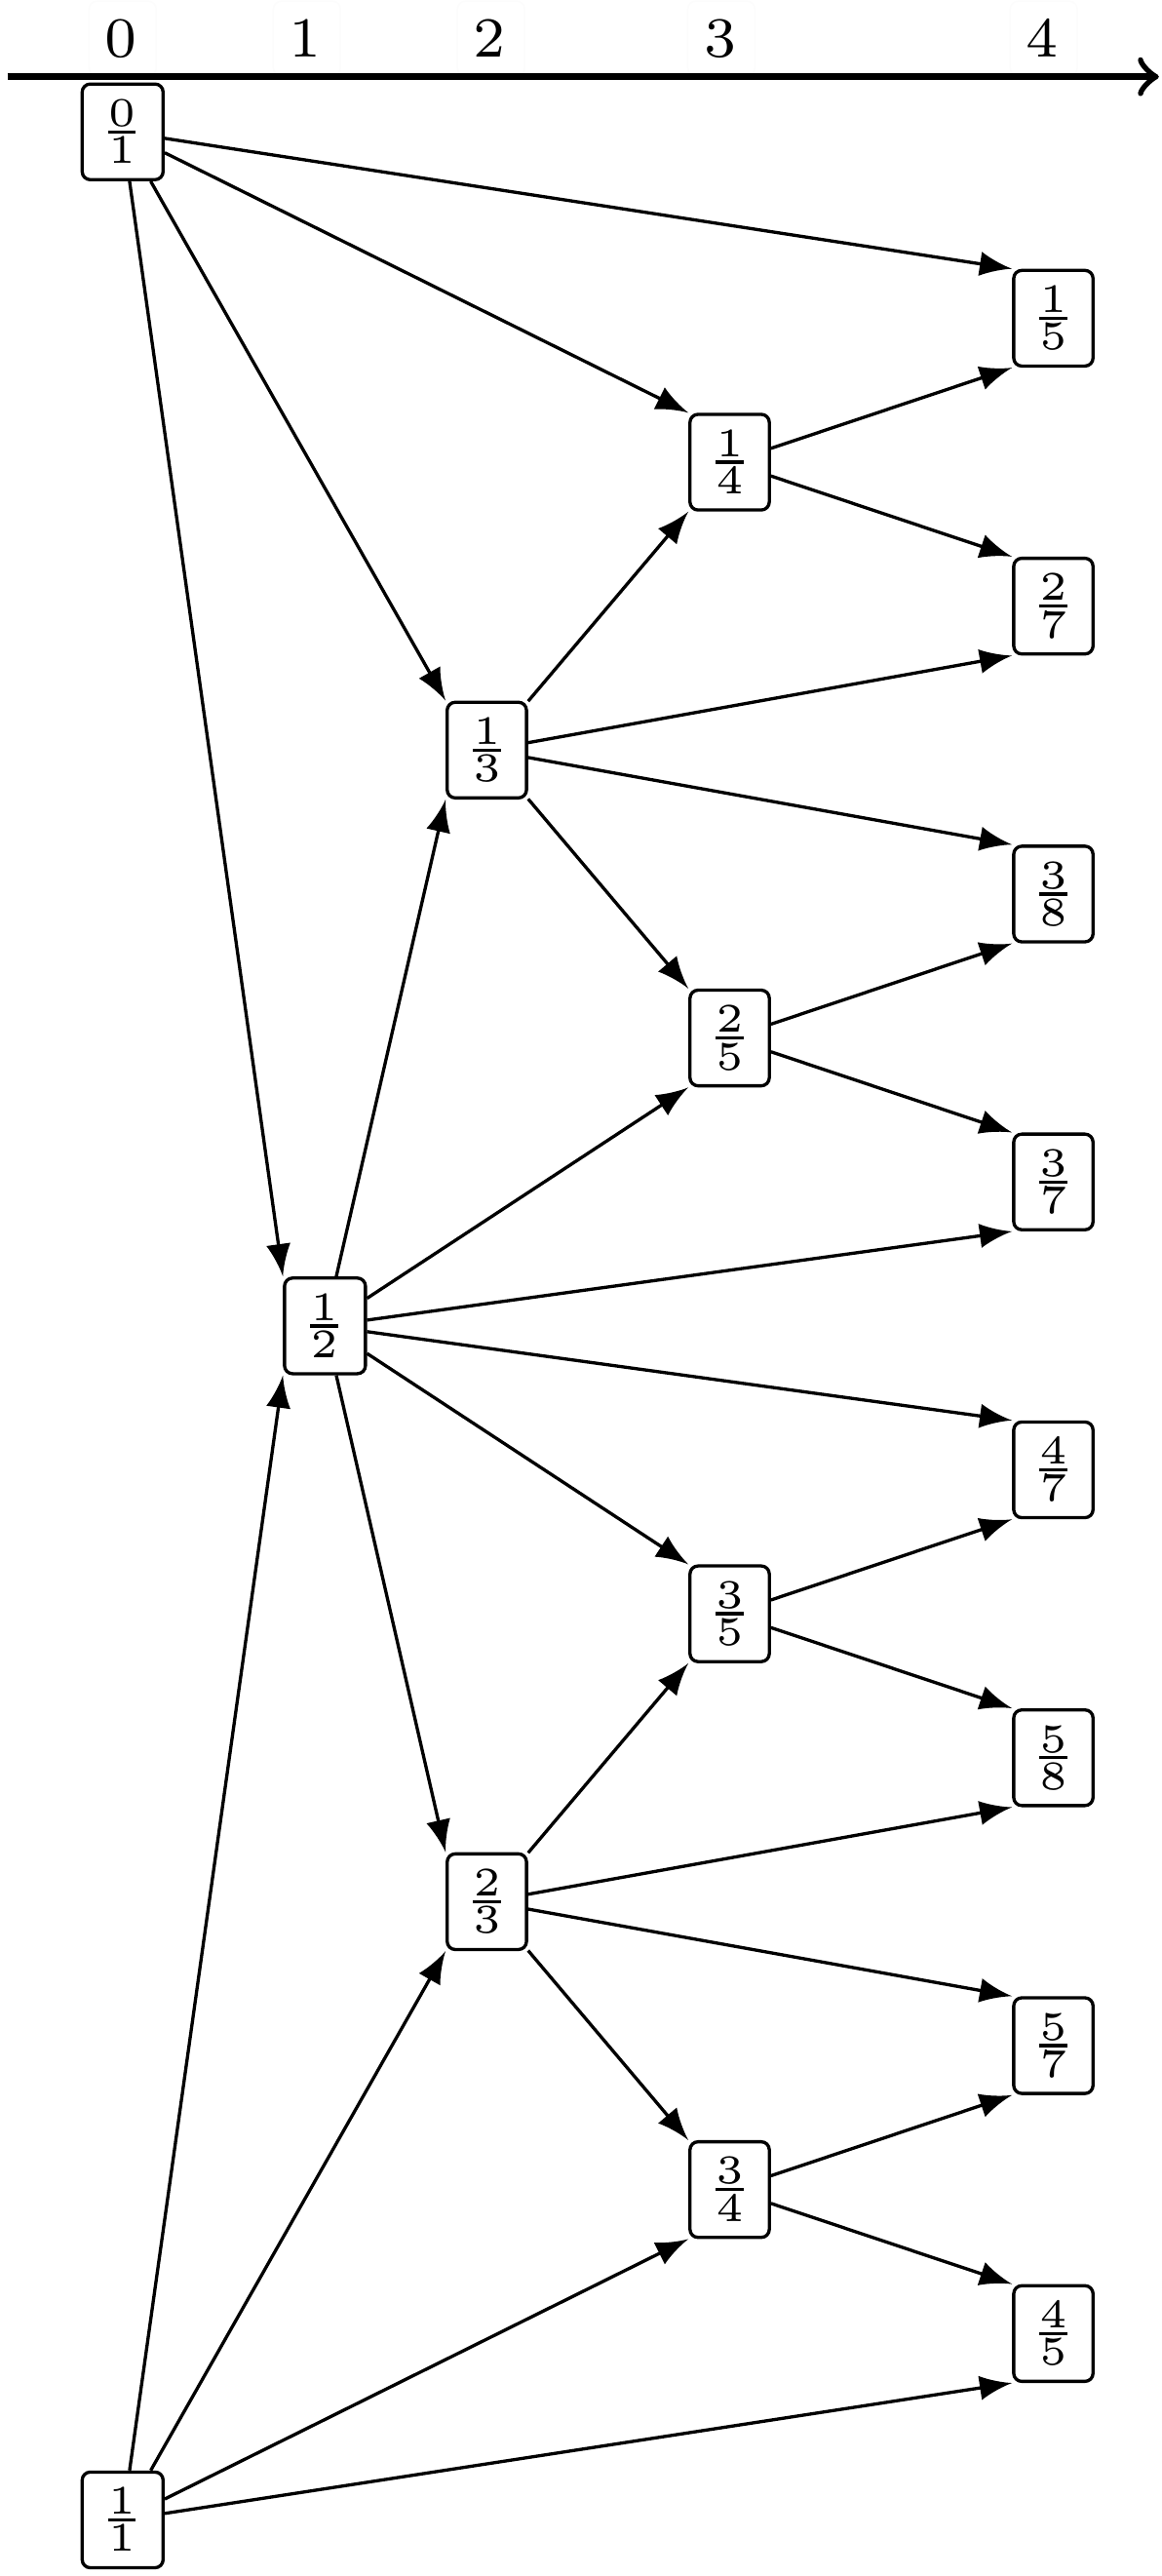
\includegraphics[width=.47 \textwidth]{../../Report/Figures/FareyTrees/LR_RotNum/adding.png}
			\end{figure}
		\end{column}
	\end{columns}
\end{frame}

\begin{frame}{Rotation Numbers}
	\vspace{-1em}
	\begin{definition}[Rotaion Numbers --- Poincaré]
		The rotation number of a cycle $\sigma$ with period $|\sigma|$ and $n$ rotations is defined as the fraction
		\begin{align*}
			\frac{n}{|\sigma|}
		\end{align*}
	\end{definition}
	\pause
	\begin{definition}[Rotation Numbers --- Keener]
		The rotation number of a cycle $\sigma$ with period $|\sigma|$ and $|\sigma|_\L$ symbols $\L$ is defined as
		\begin{align*}
			\frac{|\sigma|_\L}{|\sigma|}
		\end{align*}
	\end{definition}
	\vspace{-3em}
	\begin{flushright}
		\cite{Keener80}
	\end{flushright}
\end{frame}

\begin{frame}{Farey-trees with Rotation Numbers}
	\begin{columns}
		\begin{column}{.5 \textwidth}
			\begin{itemize}
				\item The rotation numbers of cycles in any period-adding structure of $\L$ and $\R$ are given by the same Farey-tree with starting nodes $\frac{1}{1}$ and $\frac{0}{1}$
				      \pause
				\item Why?
			\end{itemize}
		\end{column}
		\begin{column}{.5 \textwidth}
			\vspace{-5em}
			\begin{figure}
				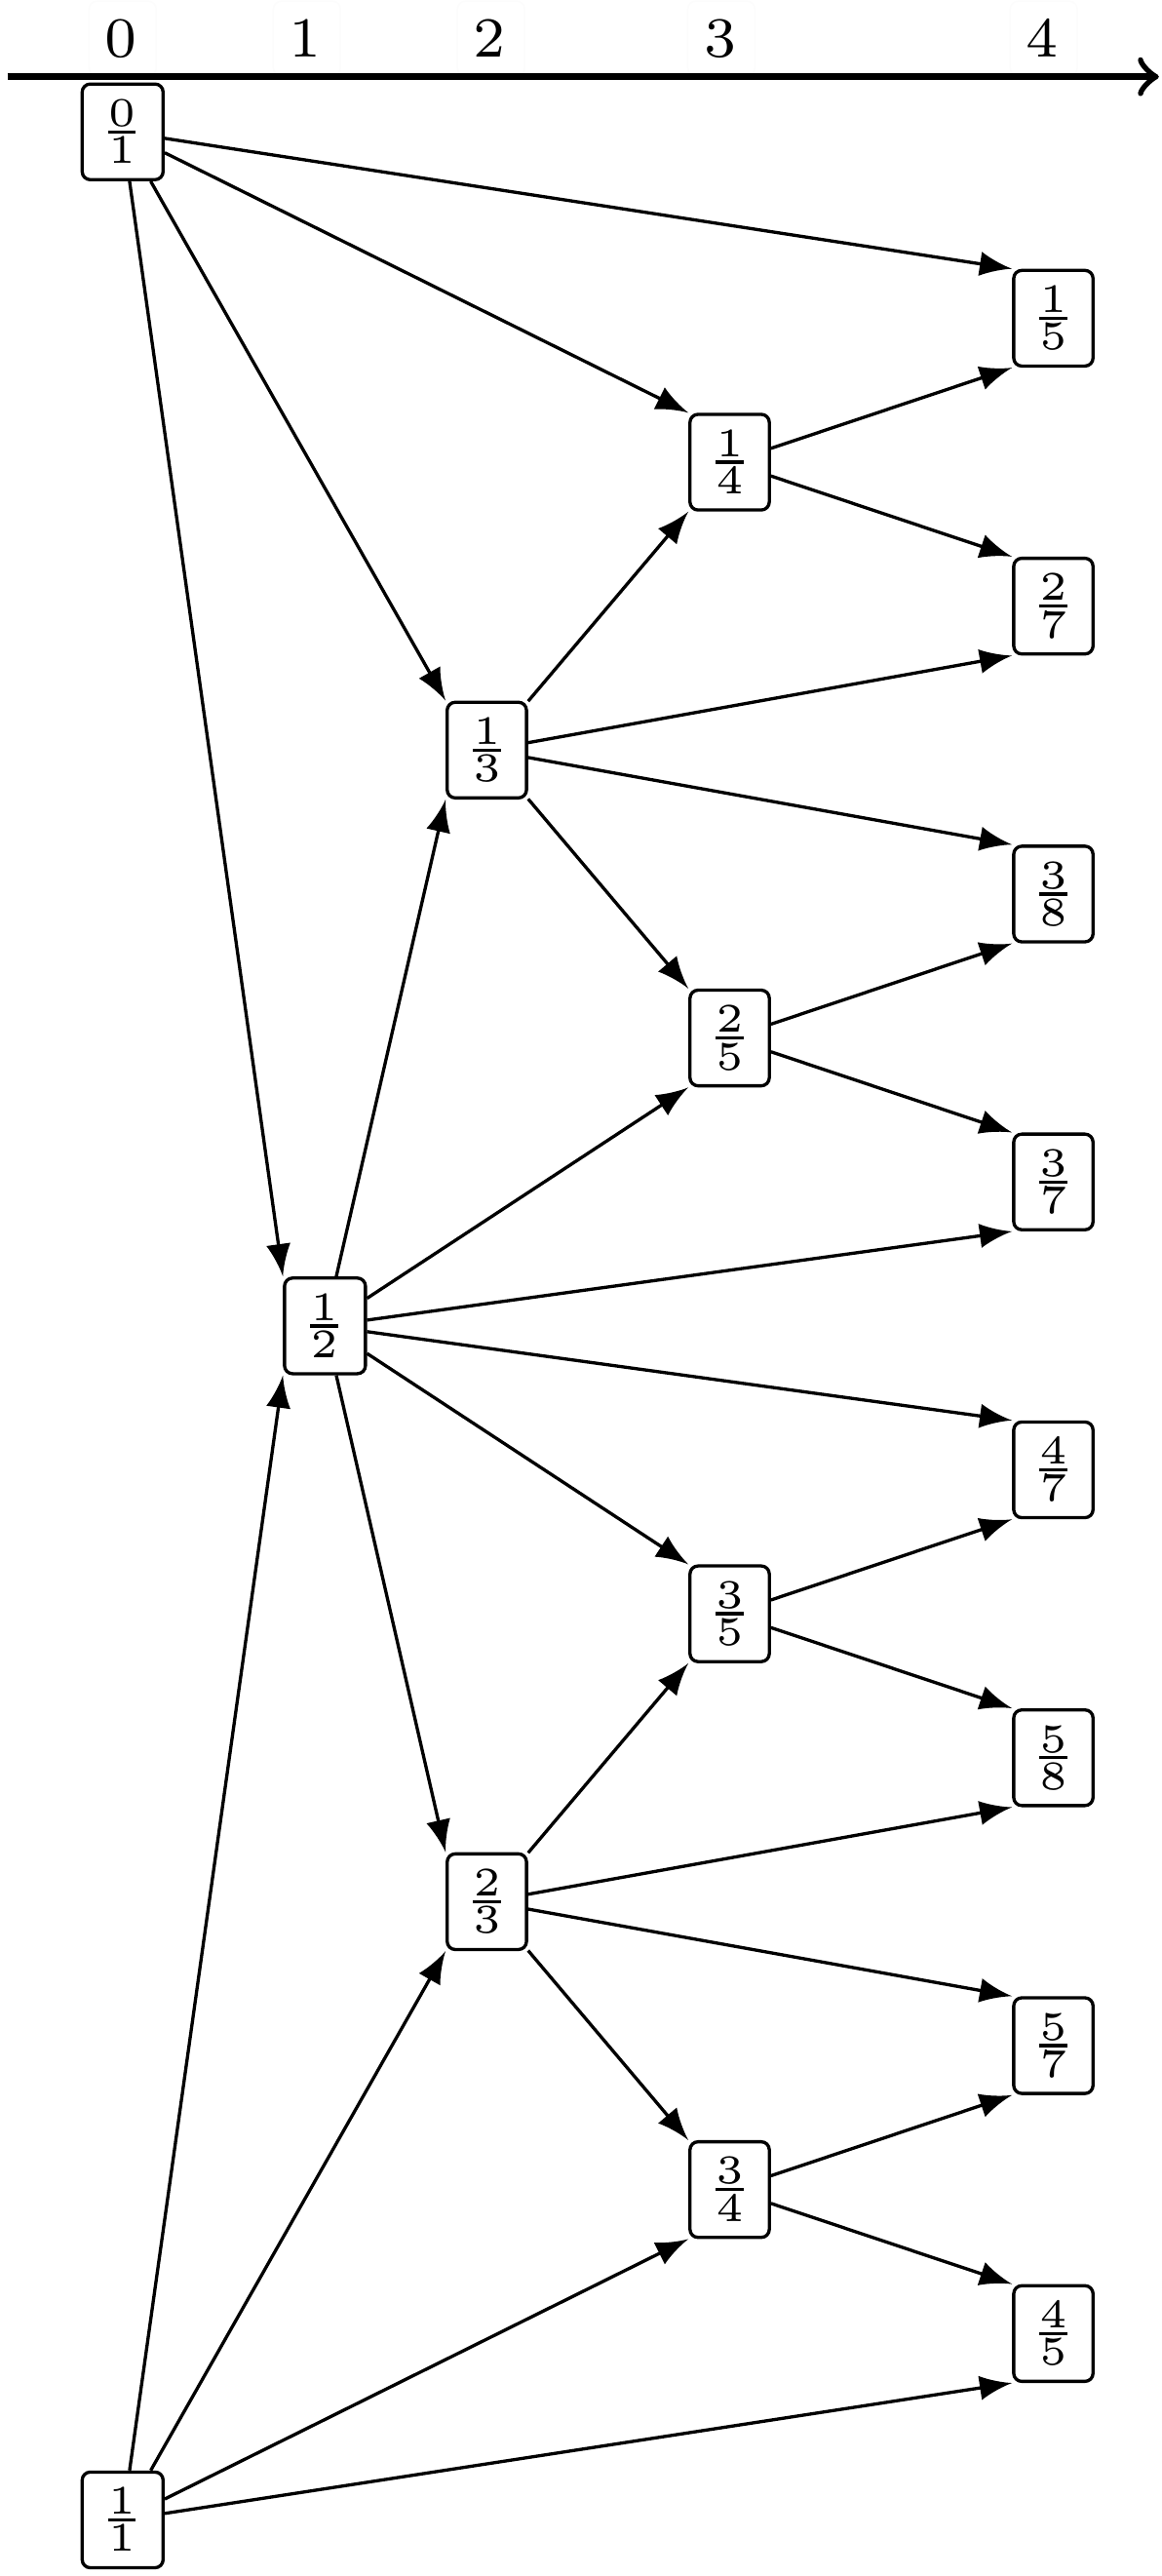
\includegraphics[width=.47 \textwidth]{../../Report/Figures/FareyTrees/LR_RotNum/adding.png}
			\end{figure}
		\end{column}
	\end{columns}
\end{frame}

\begin{frame}{Farey-trees with Symbolic Sequences}
	\begin{columns}
		\begin{column}{.5 \textwidth}
			\begin{itemize}
				\item Keep the structure of the tree
				\item Replace starting nodes with symbolic sequences $\L$ and $\R$
				\item Use concatenation instead of Farey-addition $\oplus$
			\end{itemize}
			\pause
			\vspace{2em}
			This is the rule, the symbolic sequences follow in period-adding scenarios
		\end{column}
		\begin{column}{.5 \textwidth}
			\vspace{-3em}
			\begin{figure}
				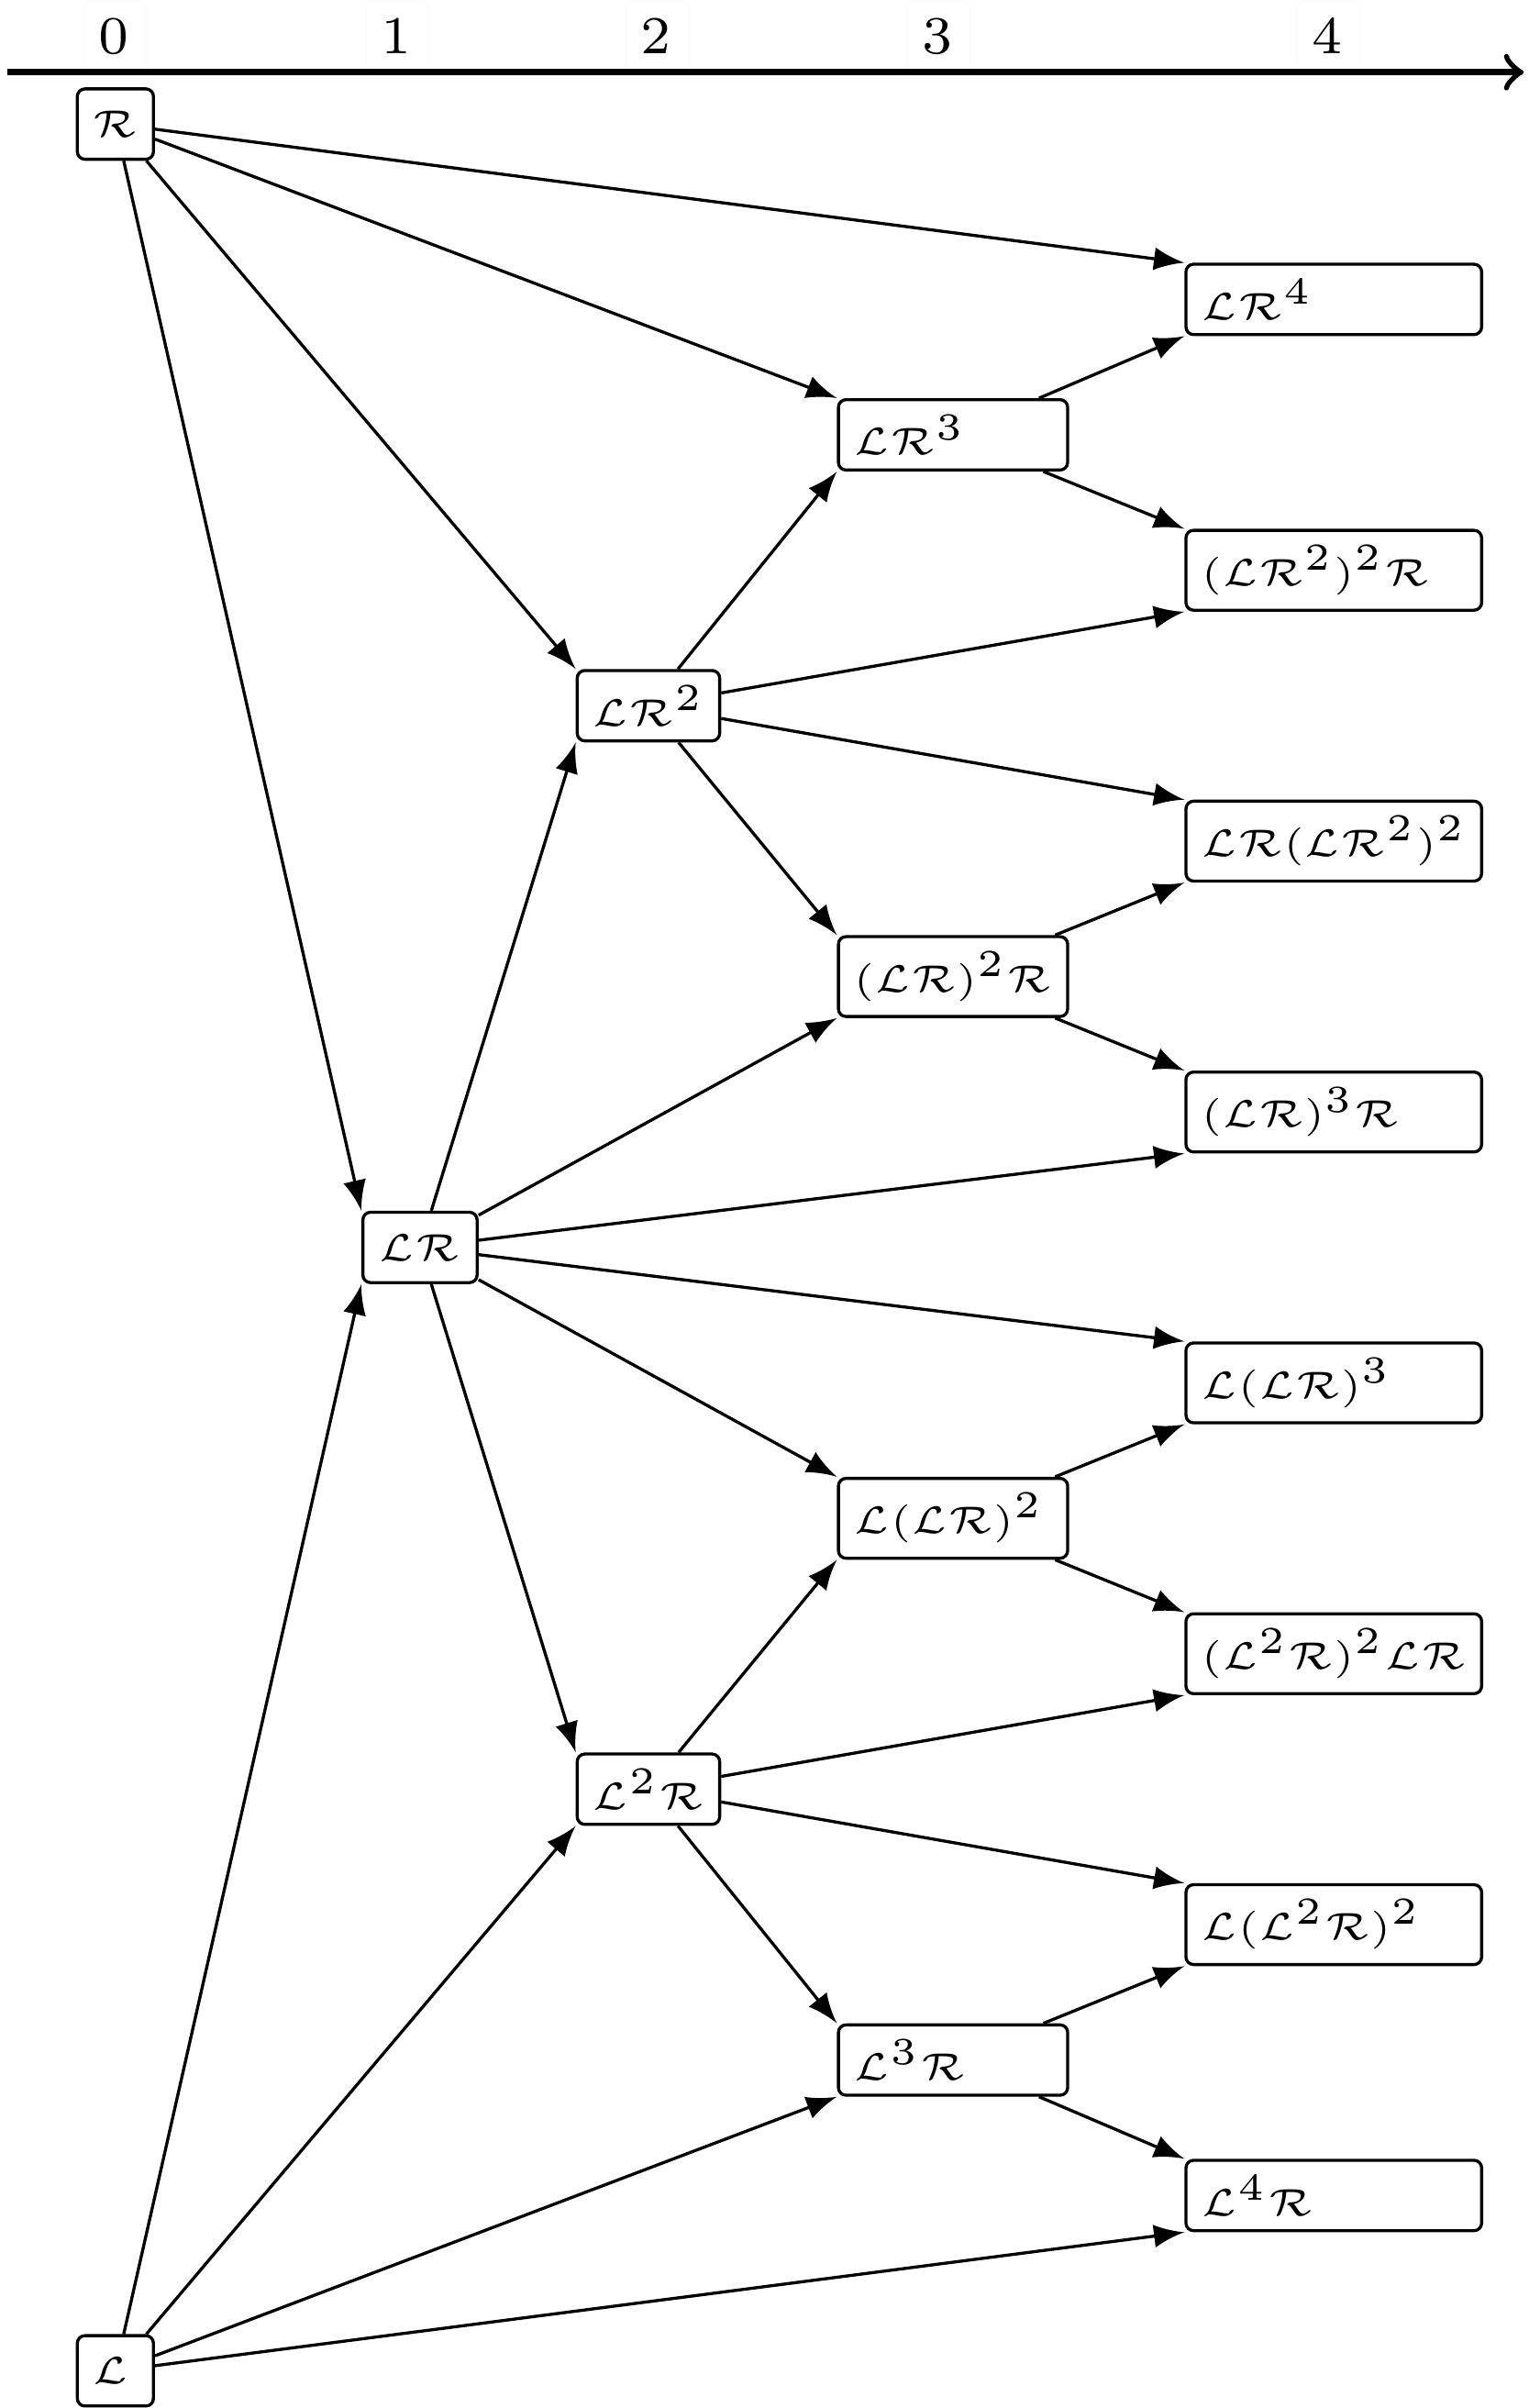
\includegraphics[width=.6 \textwidth]{../../Report/Figures/FareyTrees/LR/adding.png}
			\end{figure}
		\end{column}
	\end{columns}
\end{frame}

\begin{frame}{Concatenation and Rotation Numbers}
	\begin{theorem}[Rotation Numbers of Concatenated Cycles]
		The rotation number of the concatenated cycle $\sigma\varrho$ is the Farey-sum of the rotation numbers of the cycles $\sigma$ and $\varrho$.
		\begin{align*}
			\rho(\sigma\varrho) = \rho(\sigma) \oplus \rho(\varrho)
		\end{align*}
	\end{theorem}

	\pause
	\begin{itemize}
		\item Periods add $\Rightarrow$ denominators add
		\item Number of $\L$ symbols add $\Rightarrow$ numerators add
		\item Number of rotations add $\Rightarrow$ numerators add (Poincaré)
	\end{itemize}
\end{frame}

\begin{frame}{Concatenation and Rotation Numbers}
	\begin{figure}
		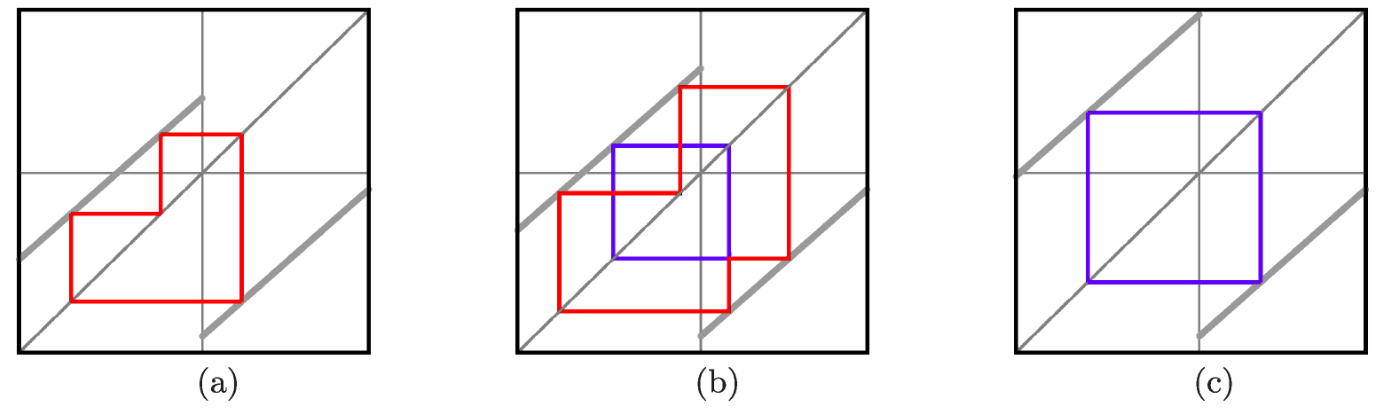
\includegraphics[width=.8 \textwidth]{Figs/PeriodAddingCobwebs_Slides.png}
	\end{figure}
	\begin{columns}
		\begin{column}{.3 \textwidth}
			\begin{itemize}
				\item Sequence: $\L^2\R$
				\item Rotation Number: $\frac{2}{3}$
			\end{itemize}
		\end{column}
		\begin{column}{.3 \textwidth}
			\begin{itemize}
				\item Sequence: $\L^2\R\L\R$
				\item Rotation Number: $\frac{3}{5}$
			\end{itemize}
		\end{column}
		\begin{column}{.3 \textwidth}
			\begin{itemize}
				\item Sequence: $\L\R$
				\item Rotation Number: $\frac{1}{2}$
			\end{itemize}
		\end{column}
	\end{columns}
\end{frame}

%\begin{frame}{Number of Branches}
%	\begin{itemize}
%		\item Simplified model has more than 2 branches
%		      \pause
%		\item[$\Rightarrow$] Tuple of 4 rotation-like numbers
%	\end{itemize}
%	\begin{definition}[Rotation Tuples]
%		For our cycles with 4 branches we define rotation tuples.
%		\begin{align*}
%			\rho(\phi)
%			= (\rho_\A(\phi), \rho_\B(\phi), \rho_\C(\phi), \rho_\D(\phi))
%			= \left(\frac{|\phi|_\A}{|\phi|}, \frac{|\phi|_\B}{|\phi|}, \frac{|\phi|_\C}{|\phi|}, \frac{|\phi|_\D}{|\phi|}\right)
%		\end{align*}
%	\end{definition}
%\end{frame}

\begin{frame}{Period Adding in Between Chains}
	\vspace{-1em}
	Period-adding is common in between chains of cycles with the same period
	\begin{figure}
		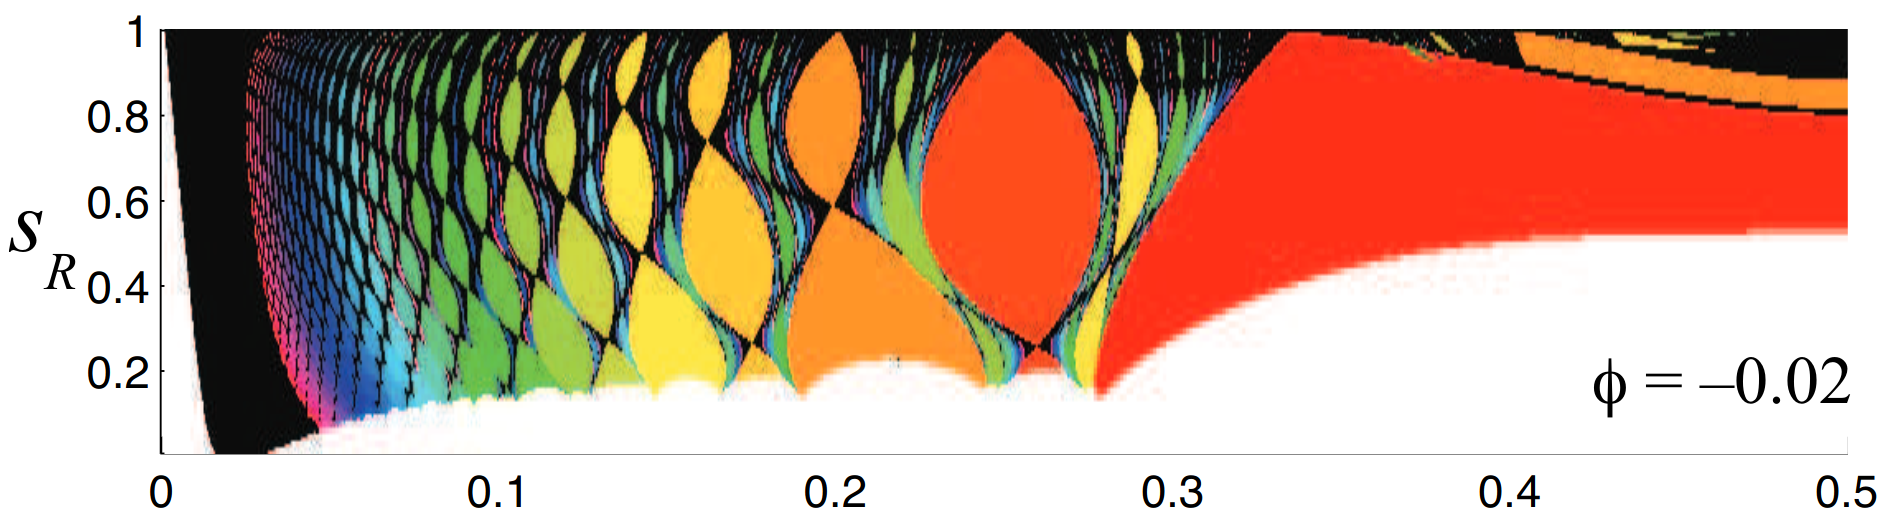
\includegraphics[width=.5 \textwidth]{Figs/tounge_adding.png}\\
		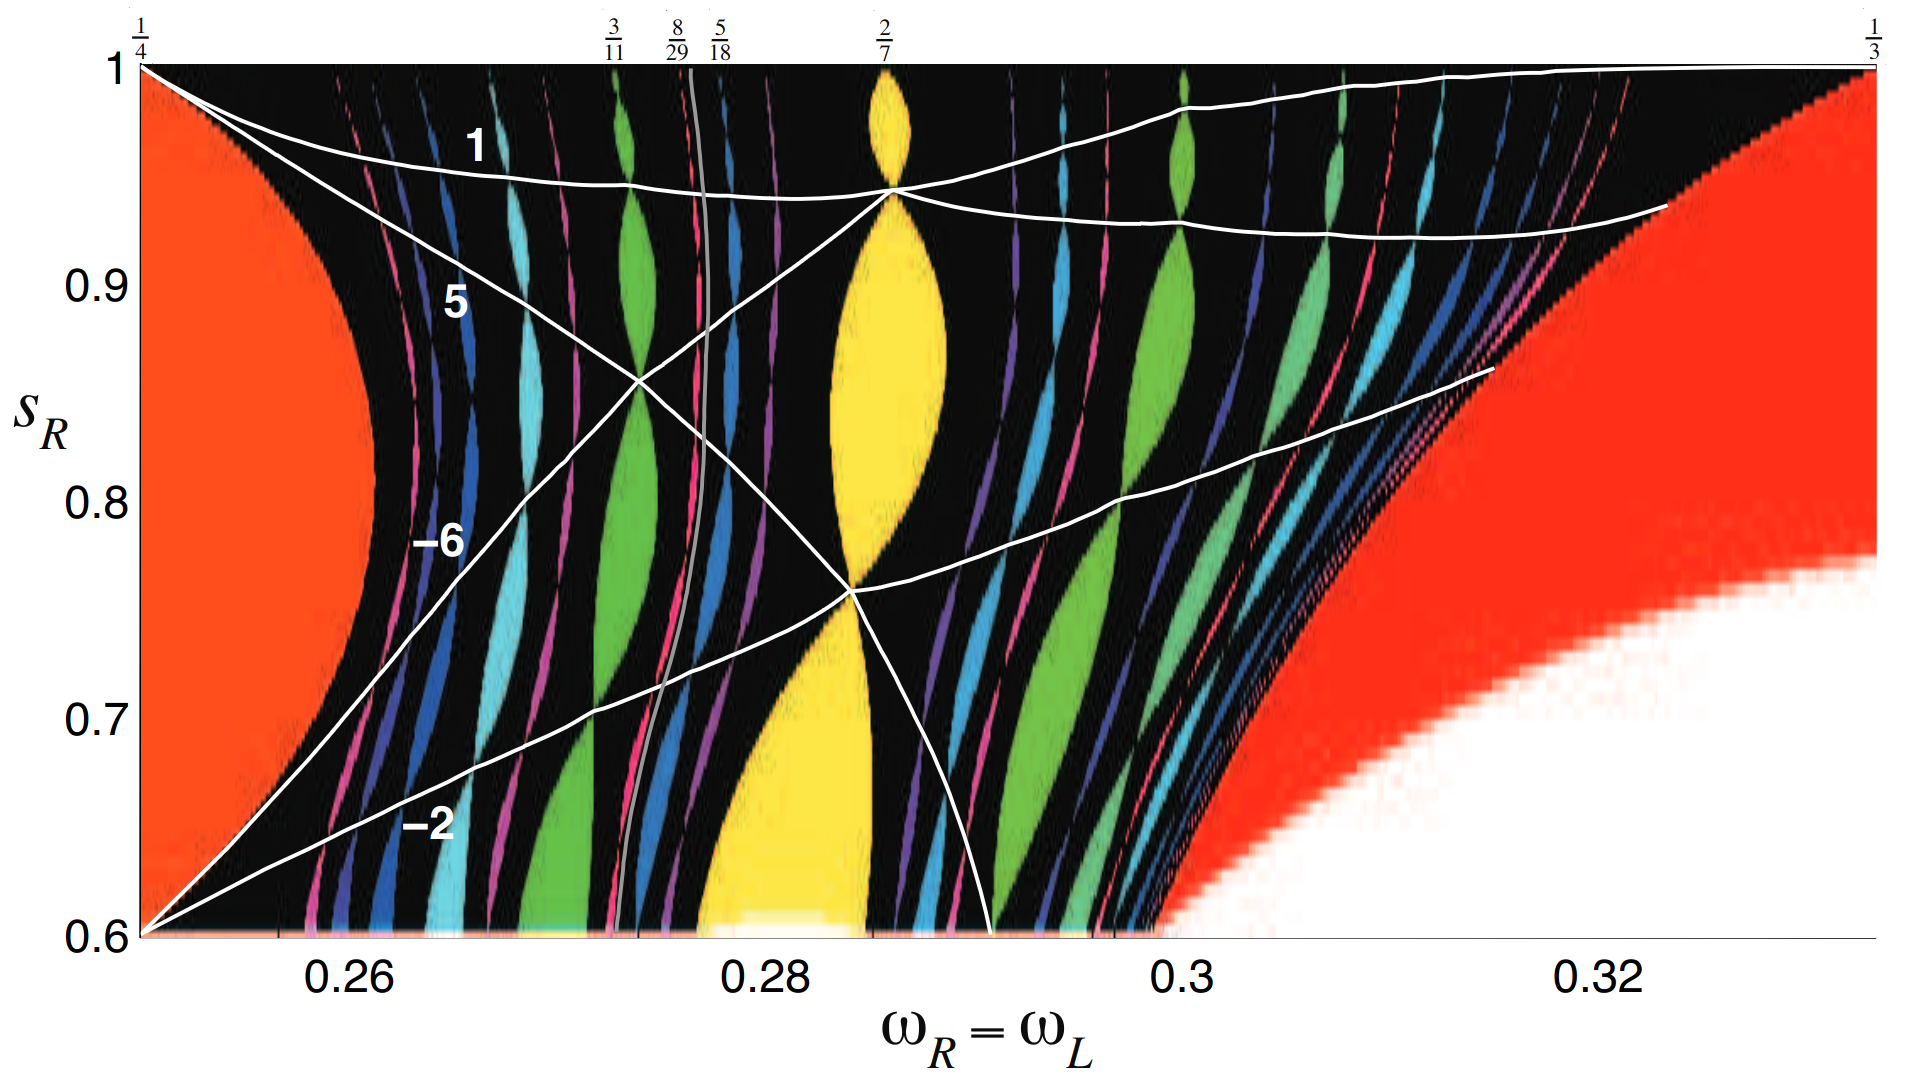
\includegraphics[width=.5 \textwidth]{Figs/tounge_adding_zoomed.png}
	\end{figure}
	\vspace{-2em}
	\begin{flushright}
		Pictures from \cite{simpson2010}
	\end{flushright}
\end{frame}
